\documentclass[2pt, a4paper, fleqn]{extarticle}

\usepackage[T2A]{fontenc}
\usepackage[utf8]{inputenc}
\usepackage[english,russian]{babel}
\usepackage{url}
%\usepackage{pscyr}

%\renewcommand{\rmdefault}{ftm}
\usepackage{setspace}
\onehalfspacing

\usepackage{changepage}
\usepackage{indentfirst} %первый абзац
%%\usepackage{moreverb}
\usepackage[noend]{algorithmic}
\usepackage{amssymb, amsmath, multicol,amsthm}
%%
\usepackage{enumitem, multicol}
\usepackage{titleps,lipsum}
%%
\usepackage{mathrsfs}
\usepackage{verbatim}
\usepackage{pb-diagram}
\usepackage{graphicx}
\graphicspath{ {images/} }
\usepackage{wrapfig}
\usepackage{xcolor}
\definecolor{new}{RGB}{255,184,92}
\definecolor{news}{RGB}{112,112,112}
\usepackage{wallpaper}
\usepackage{float}
\usepackage{hyperref}
\hypersetup{
%colorlinks=true,%
%linkcolor=news,%
linkbordercolor=new,
}



\usepackage{geometry}
\geometry{top=1cm,bottom=2cm,left=1cm,right=1cm}

%\flushbottom
%\ruggedbottom

\binoppenalty=5000
\parindent=0pt

\newcommand{\EDS}{\ensuremath{\mathscr{E}}}
\newcommand*{\hm}[1]{#1\nobreak\discretionary{}%
{\hbox{$\mathsurround=0pt #1$}}{}}
\newcommand{\divisible}{\mathop{\raisebox{-2pt}{\vdots}}}
\renewcommand{\theequation}{\arabic{equation}}
\def\hm#1{#1\nobreak\discretionary{}{\hbox{$#1$}}{}}
\newcommand{\bbskip}{\bigskip \bigskip}



%%\DeclareMathOperator{\tg}{tg}
%%\DeclareMathOperator{\ctg}{ctg}

\let\leq\leqslant
\let\geq\geqslant



% Remove brackets from numbering in List of References
\makeatletter
\renewcommand{\@biblabel}[1]{\quad#1.}
\makeatother

\begin{document}

{\bf I.} Уравнение, решаемое на первом шаге: $$\dfrac{\partial n_i}{\partial t} = \dfrac{\partial}{\partial z}\bigg[D\sin^2 I \bigg(\dfrac{\partial n_i}{\partial z}+\left(\dfrac{1}{T_p}\dfrac{\partial T_p}{\partial z}+\dfrac{1}{H}\right)n_i\bigg)-\dfrac{1}{a}D\sin I\cos I\left(\dfrac{\partial n_i}{\partial\varphi}+\dfrac{1}{T_p}\dfrac{\partial T_p}{\partial \varphi}n_i\right)\bigg]+[P-kn_i]$$


Во всех случаях используем для диффузионного слагаемого схему, получаемую применением формулы центральной разности дважды, а для потокового слагаемого $\dfrac{\partial}{\partial z} (un)$ центральную разность. Вычисление $u_\varphi$ ведётся по формуле $$u_\varphi \approx -\dfrac{1}{a}\cos I \sin I\dfrac{2}{n_{i, j+1}^t+n_{i, j-1}^t}\begin{cases}\dfrac{n_{i, j+1}^t+n_{i, j}^t}{\Delta\varphi}, \sin I \geq 0\\\dfrac{n_{i, j}^t+n_{i, j-1}^t}{\Delta\varphi}, \sin I \leq 0 .\end{cases}$$

Полная схема для уравнения на первом шаге: 

$$\dfrac{n_{i,j}^{t+1}-n_{i,j}^t}{\tau} = P - k n_{i, j}^{t+1} + \bigg[\left(D_{i+1/2}\dfrac{n_{i+1, j}^{t+1}-n_{i,j}^{t+1}}{h^2}-D_{i-1/2}\dfrac{n_{i,j}^{t+1}-n_{i-1,j}^{t+1}}{h^2}\right)+\left(\dfrac{u_{i+1}n_{i+1,j}^{t+1}-u_{i-1}n_{i-1,j}^{t+1}}{2h}\right) +$$ $$+ \left(\dfrac{u_{\varphi(i+1/2)}+|u_{\varphi(i+1/2)}|}{2h}n_{i,j}^{t+1}+\dfrac{u_{\varphi(i+1/2)}-|u_{\varphi(i+1/2)}|}{2h} n_{i+1,j}^{t+1}-\dfrac{u_{\varphi(i-1/2)}+|u_{\varphi(i-1/2)}|}{2h}n_{i-1,j}^{t+1}-\dfrac{u_{\varphi(i-1/2)}-|u_{\varphi(i-1/2)}|}{2h} n_{i,j}^{t+1}\right) \bigg]$$

На верхней границе учитывается равенство нулю полного потока: в результате имеем уравнение: 
$$\dfrac{n_{i,j}^{t+1}-n_{i,j}^t}{\tau} = + \bigg[-D_{i-1/2}\dfrac{n_{i,j}^{t+1}-n_{i-1,j}^{t+1}}{h^2}-\left(\dfrac{u_{i}n_{i,j}^{t+1}+u_{i-1}n_{i-1,j}^{t+1}}{2h}\right) +$$ $$+ \left(-\dfrac{u_{\varphi(i-1/2)}+|u_{\varphi(i-1/2)}|}{2h}n_{i-1,j}^{t+1}-\dfrac{u_{\varphi(i-1/2)}-|u_{\varphi(i-1/2)}|}{2h} n_{i,j}^{t+1}\right) \bigg]$$

На нижней границе $n_{i, j}^{t+1} = P/k$.

На граничных точках $\varphi = \pm 89{,}5^\circ$ коэффициент $\sin I$ перед смешанной производной мал. Для того, чтобы избавиться от необходимости использовать при подсчете $u_\varphi$ значения с предыдущего временного шага, находящиеся вне рассматриваемой расчетной области, в этих граничных точках сетки из уравнения системы исключены слагаемые со смешанной производной:
$$\dfrac{n_{i,j}^{t+1}-n_{i,j}^t}{\tau} = P - k n_{i, j}^{t+1} + \bigg[\left(D_{i+1/2}\dfrac{n_{i+1, j}^{t+1}-n_{i,j}^{t+1}}{h^2}-D_{i-1/2}\dfrac{n_{i,j}^{t+1}-n_{i-1,j}^{t+1}}{h^2}\right)+\left(\dfrac{u_{i+1}n_{i+1,j}^{t+1}-u_{i-1}n_{i-1,j}^{t+1}}{2h}\right) \bigg]$$


\bigskip

{\bf II.} Уравнение, решаемое на втором шаге расщепления:

$$\dfrac{\partial n}{\partial t} = \dfrac{1}{a\cos\varphi} \dfrac{\partial }{\partial \varphi}\left[\dfrac{D}{a}\cdot(\cos^2  I \cos\varphi)\cdot\dfrac{\partial n}{\partial \varphi}-D\cdot(\sin I\cos I\cos\varphi)\cdot \dfrac{\partial n}{\partial z} - u\cdot(\sin I \cos I \cos\varphi)\cdot n \right]$$

Здесь $u = D\left(\dfrac{1}{T_p}\dfrac{\partial T_p}{\partial z}+\dfrac{1}{H}\right)$~---~эффективная скорость из первого шага, $I = \arctg(2\tg \varphi)$.

В качестве начальных условий выступает решение уравнения с первого шага расщепления. Введём две функции: $$A(\varphi) = \cos \varphi \cdot \cos^2(\arctg(2\tg \varphi)) = \dfrac{\cos\varphi}{1+4\tg^2\varphi}\mbox{ и }B(\varphi) = \cos\varphi \cdot \sin(2\arctg(2\tg \varphi))=\dfrac{4\sin\varphi}{1+4\tg^2\varphi}.$$

С помощью этих функций задачу можно переписать в следующем виде: 
$$\dfrac{\partial n}{\partial t} = \dfrac{1}{\cos\varphi} \dfrac{\partial }{\partial \varphi}\left[\dfrac{D}{a^2}A(\varphi)\dfrac{\partial n}{\partial \varphi}-\dfrac{D}{2a}B(\varphi) \dfrac{\partial n}{\partial z} - \dfrac{u}{2a}B(\varphi) n \right]$$

Для полного уравнения используем следующую схему:
$$\dfrac{n_{i,j}^{t+1}-n_{i,j}^t}{\tau} = \dfrac{1}{\cos\varphi_j} \bigg[\dfrac{D}{a^2}\left(A(\varphi_{j+1/2})\dfrac{n_{i, j+1}^{t+1}-n_{i,j}^{t+1}}{\Delta\varphi^2}-A(\varphi_{j-1/2})\dfrac{n_{i,j}^{t+1}-n_{i,j-1}^{t+1}}{\Delta\varphi^2}\right)-$$ $$-\dfrac{u}{2a}\left(\dfrac{B(\varphi_{j+1})n_{i,j+1}^{t+1}-B(\varphi_{j-1})n_{i,j-1}^{t+1}}{2\Delta\varphi}\right) - MIX_{\varphi, z}(n)_{i, j}^{t+1} \bigg]$$

Здесь $MIX_{\varphi, z}(n)_{i, j}^{t+1}$~---~аппроксимация смешанной производной $MIX_{\varphi, z}(n) = \dfrac{-1}{\cos\varphi}\dfrac{\partial }{\partial\varphi}\left(\dfrac{D}{2a}u_z n\right) $, где введено обозначение $u_z = B(\varphi)\dfrac{1}{n}\dfrac{\partial n}{\partial z} = B(\varphi)\dfrac{\partial \ln n}{\partial z}$. При этом значения $n$ для вычисления $u_z$ берутся с предыдущего временного шага. Аналогично первому шагу, $$u_z \approx B(\varphi)\dfrac{2}{n_{i+1, j}^t+n_{i-1, j}^t}\begin{cases}\dfrac{n_{i+1, j}^t+n_{i, j}^t}{h}, B(\varphi) \geq 0\\\dfrac{n_{i, j}^t+n_{i-1, j}^t}{h}, B(\varphi) \leq 0 .\end{cases}$$

После вычисления $u_z$ в узлах $(i, j)$, $(i, j+1)$, $(i, j-1)$ в зависимости от знака произведения $\cos\varphi \cdot u_{z(i, j)}$ аппроксимируется смешанная производная :  $$MIX_{\varphi, z}(n)_{i, j} \approx \begin{cases}\dfrac{u_{z(i, j+1)}n_{i, j+1}^{t+1} - u_{z(i, j)}n_{i, j}^{t+1}}{\Delta\varphi}, (-u_{z(i, j)}\cos\varphi) \geq 0\\ \dfrac{u_{z(i, j)}n_{i, j}^{t+1} - u_{z(i, j-1)}n_{i, j-1}^{t+1}}{\Delta\varphi}, (-u_{z(i, j)}\cos\varphi) \leq 0 .\end{cases}$$

При $i = 1$ $(z = 100\mbox{ } \mbox{км})$ также ставим граничное условие Дирихле~---~на нижней границе по $z$ решение совпадает с полученным на первом шаге.

На верхней границе требуется граничное условие для определения $u_z$.

Поток на границе $z=z_{ub}$: $$\dfrac{D}{a^2}A(\varphi_{j+1/2})\dfrac{n_{N, j+1}-n_{N, j}}{h}-\dfrac{u}{2a}\dfrac{B(\varphi_{j+1})n_{N, j+1}+B(\varphi_j)n_{N, j}}{2\Delta\varphi}-$$ $$-\dfrac{D}{2a}\left(\dfrac{u_{z(j+1/2)}+|u_{z(j+1/2)}|}{2\Delta\varphi}n_{i,j}^{t+1}+\dfrac{u_{z(j+1/2)}-|u_{z(j+1/2)}|}{2\Delta\varphi} n_{i,j+1}^{t+1}\right) = F_{y}\approx 0$$
С помощью условия равенства нулю потока на границе $z = 500$~км получаем, что при решении линейной системы во втором шаге расщепления сохраняются значения при $z = 500$~км с первого шага расщепления, т.~е. в рамках решения уравнения второго шага расщепления имеет место граничное условие Дирихле на этой границе: равенство результату с первого шага.

При $j = 1$ $(\varphi = -89{,}5^\circ)$ и $j = N_\varphi$ $(\varphi = +89{,}5^\circ)$ используем следующее граничное условие: в точках $(i, j+1/2)$ на северном полюсе и $(i, j-1/2)$ на южном функции $A(\varphi)$ и $B(\varphi)$ имеют нули третьего и второго порядка соответственно, что позволяет занулить на этих слоях по $j$ те слагаемые, в которых множители $A$ и $B$ берутся на полюсах.

Это означает, что при $j = 1$ используется аппроксимация $$\dfrac{n_{i,j}^{t+1}-n_{i,j}^t}{\tau} = \dfrac{1}{\cos\varphi_j} \bigg[\dfrac{D}{a^2}\left(A(\varphi_{j+1/2})\dfrac{n_{i, j+1}^{t+1}-n_{i,j}^{t+1}}{\Delta\varphi^2}\right)-\dfrac{u}{2a}\left(\dfrac{B(\varphi_{j+1})n_{i,j+1}^{t+1}+B(\varphi_{j})n_{i,j}^{t+1}}{2\Delta\varphi}\right) -MIX_{\varphi, z}(n)_{i, j}^{t+1}\bigg) \bigg]$$
Аналогично, на северном полюсе при $j=N_\varphi$: $$\dfrac{n_{i,j}^{t+1}-n_{i,j}^t}{\tau} = \dfrac{1}{\cos\varphi_j} \bigg[\dfrac{D}{a^2}\left(-A(\varphi_{j-1/2})\dfrac{n_{i,j}^{t+1}-n_{i,j-1}^{t+1}}{\Delta\varphi^2}\right)+\dfrac{u}{2a}\left(\dfrac{B(\varphi_{j})n_{i,j}^{t+1}+B(\varphi_{j-1})n_{i,j-1}^{t+1}}{2\Delta\varphi}\right) -MIX_{\varphi, z}(n)_{i, j}^{t+1}\bigg) \bigg]$$
Аппроксимации смешанных производных $MIX_{\varphi, z}(n)_{i, j}^{t+1}$ в околополюсных точках такие же, как и внутри расчетной области, за исключением единственного отличия: на северном полюсе $u_{z(i, j-1)}$ полагается равным нулю, а на южном, при $j = N_{\varphi}$, соответственно, $u_{z(i, j+1)} = 0$.

Результаты расчетов показывают, что для устойчивого счёта при $80$ узлах по высоте и $180$ узлах по широте ($h = 5$ км, $\varphi = 1^\circ$) требуется брать шаг по времени $\tau < 160$~с.

\bigskip

{\bf Дополнение.} Исследуем асимптотическое поведение функций $A(\varphi)$ и $B(\varphi)$ вблизи полюсов (при $\varphi = \pm\dfrac{\pi}{2}$).


Имеют место следующие разложения при $\varphi\rightarrow\dfrac{\pi}{2}$: $$A(\varphi)=-\dfrac{1}{4}\cdot\left(\varphi-\dfrac{\pi}{2}\right)^3-\dfrac{1}{16}\cdot\left(\varphi-\dfrac{\pi}{2}\right)^5+o\left(\left(\varphi-\dfrac{\pi}{2}\right)^6\right)$$ $$B(\varphi) = 1\cdot\left(\varphi-\dfrac{\pi}{2}\right)^2-\dfrac{1}{12}\cdot \left(\varphi-\dfrac{\pi}{2}\right)^4+o\left(\left(\varphi-\dfrac{\pi}{2}\right)^5\right)$$

Соответственно, при $x\rightarrow-\dfrac{\pi}{2}$: $$A(\varphi)=\dfrac{1}{4}\cdot\left(\varphi+\dfrac{\pi}{2}\right)^3+\dfrac{1}{16}\cdot\left(\varphi+\dfrac{\pi}{2}\right)^5+o\left(\left(\varphi+\dfrac{\pi}{2}\right)^6\right)$$ $$B(\varphi) = -1\cdot\left(\varphi+\dfrac{\pi}{2}\right)^2+\dfrac{1}{12}\cdot \left(\varphi+\dfrac{\pi}{2}\right)^4+o\left(\left(\varphi+\dfrac{\pi}{2}\right)^5\right)$$


Графики функций $A$ и $B$ приведены ниже: 

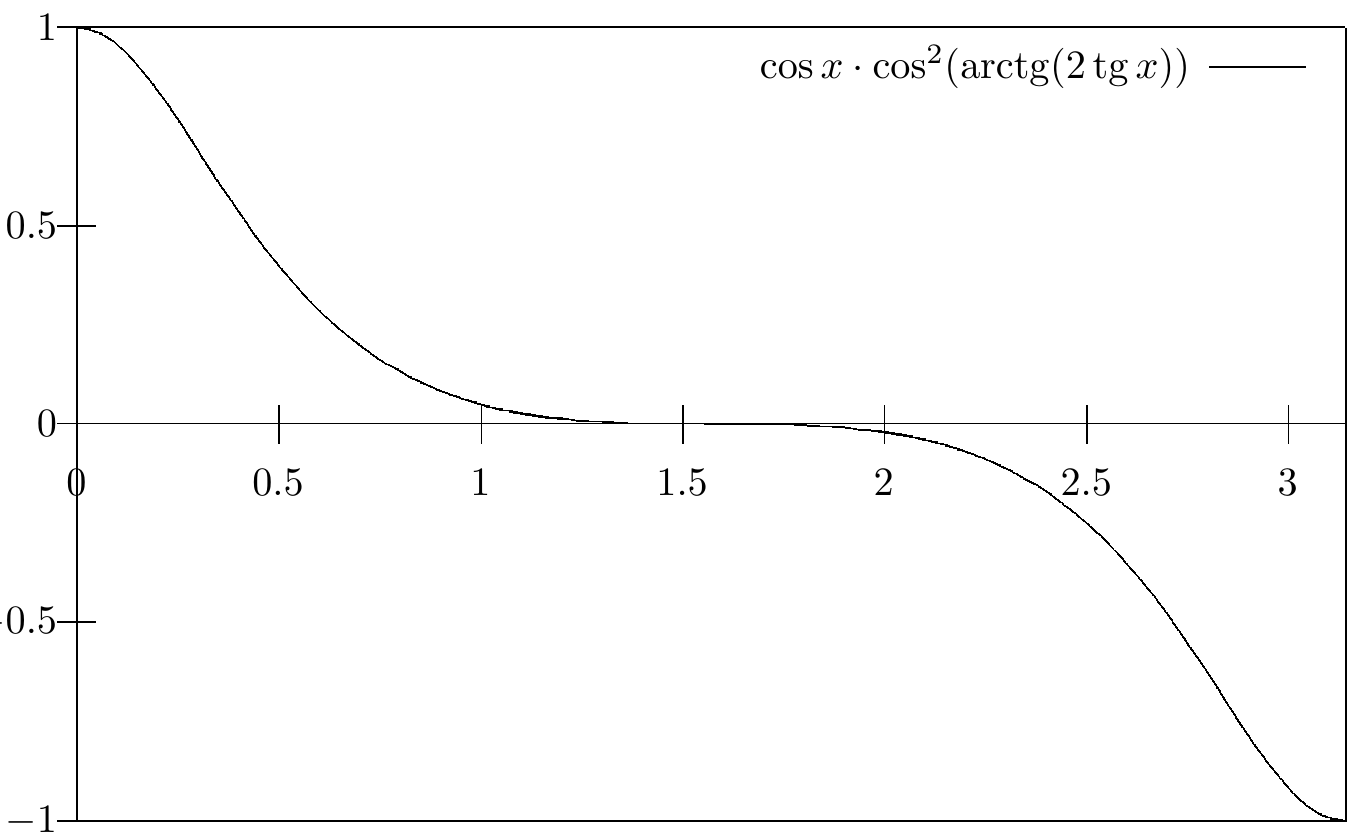
\includegraphics[scale=0.25]{A}

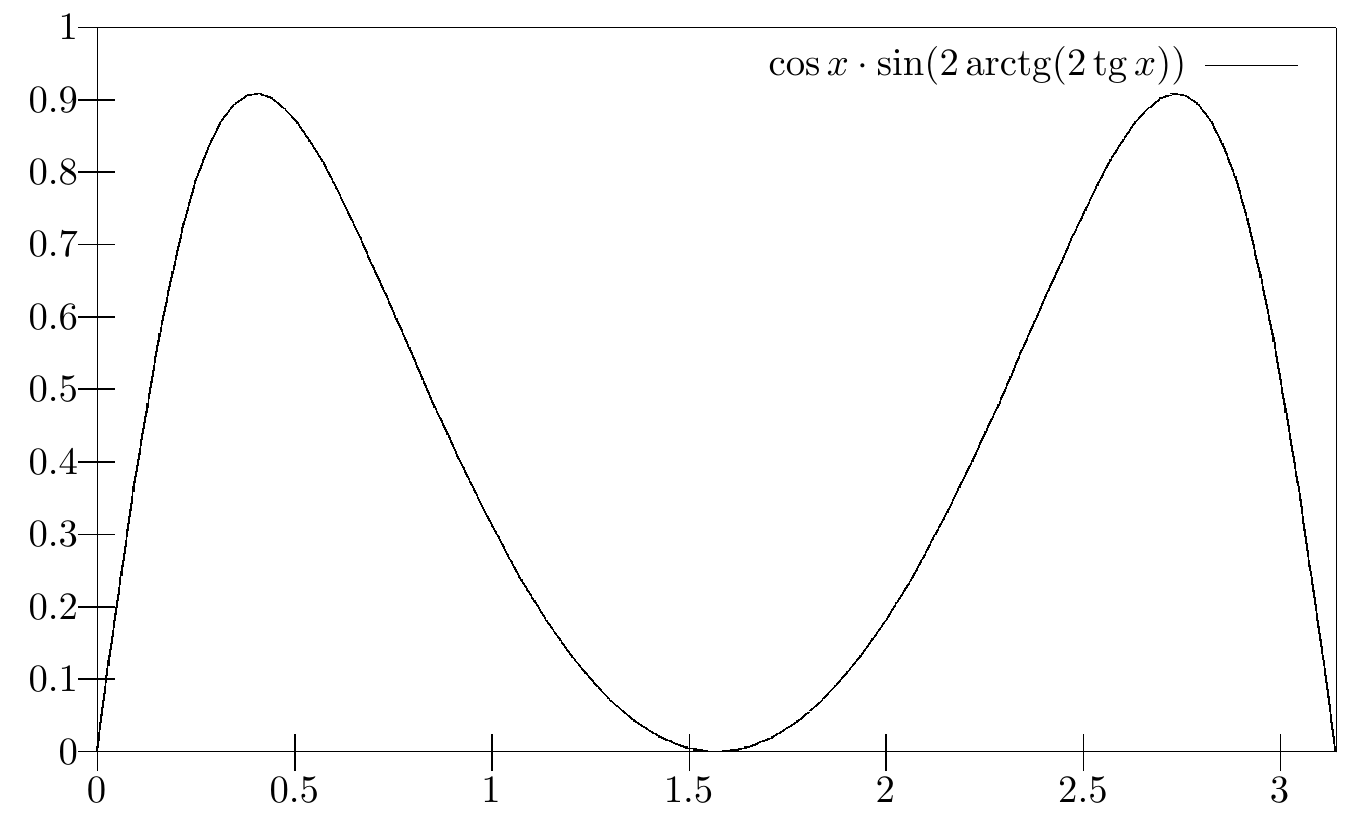
\includegraphics[scale=0.25]{B}

Обе функции в точке $\varphi = \dfrac{\pi}{2}$ касаются оси абсцисс~---~имеют нули по крайней мере второго порядка, поэтому особенность в уравнении устранимая.
\end{document}



